\part{HOL~4 History and Architecture}

\frame[plain]{\partpage}

\section{LCF}

\begin{frame}
\frametitle{LCF - Logic of Computable Functions}

\begin{itemize}
\item \emph{Standford LCF} 1971-72 by Milner et al.
\item formalism devised by Dana Scott in 1969
\item intended to reason about recursively defined functions 
\item intended for computer science applications
\item strengths
\begin{itemize}
\item powerful simplification mechanism
\item support for backward proof
\end{itemize}
\item limitations
\begin{itemize}
\item proofs need a lot of memory
\item fixed, hard-coded set of proof commands
\end{itemize}
\end{itemize}
\end{frame}

\begin{frame}
\frametitle{LCF - Logic of Computable Functions II}

\begin{itemize}
\item Milner worked on improving LCF in Edinburgh
\item research assistants
\begin{itemize}
\item Lockwood Morris
\item Malcolm Newey
\item Chris Wadsworth
\item Mike Gordon
\end{itemize}
\item \emph{Edinburgh LCF} 1979
\item introduction of \emph{Meta Language} (ML)
\item ML was invented to write proof procedures
\item ML became an influential functional programming language
\item using ML allowed implementing the \emph{LCF approach}
\end{itemize}
\end{frame}


\begin{frame}
\frametitle{LCF Approach}

\begin{itemize}
\item implement an abstract datatype \alert{thm} to represent theorems
\item semantics of ML ensure that values of type thm can only be created using its interface
\item interface is very small
\begin{itemize}
\item predefined theorems are axioms
\item function with result type theorem are inferences
\end{itemize}
\item interface is carefully designed and checked
\begin{itemize}
\item size of interface and implementation allow careful checking
\item one checks that the interface really implements only axioms and inferences that are valid in the used logic
\end{itemize}
\item \emph{However you create a theorem, there is a proof for it.}
\item together with similar abstract datatypes for types and terms, this forms the \alert{kernel}
\end{itemize}
\end{frame}


\begin{frame}
\frametitle{LCF Approach II}

\begin{exampleblock}{Modus Ponens Example}
\begin{columns}
\begin{column}{.4\textwidth}
\textbf{Inference Rule}\\\medskip
\inferrule{\Gamma \vdash a \Rightarrow b \\ \Delta \entails a}{\Gamma \cup \Delta \entails b}
\end{column}
\begin{column}{.5\textwidth}
\textbf{SML function}\\\medskip
\texttt{val MP\ :\ thm -> thm -> thm}
$\texttt{MP} (\Gamma \vdash a \Rightarrow b) (\Delta \entails a) = (\Gamma \cup \Delta \entails b)$
\end{column}
\end{columns}
\end{exampleblock}

\begin{itemize}
\item very trustworthy --- only the small kernel needs to be trusted
\item efficient --- no need to store proofs
\begin{block}{Easy to extend and automate}
However complicated and potentially buggy your code is, if a value of type theorem is produced, it has been created through the small trusted interface. Therefore the statement really holds.
\end{block}
\end{itemize}
\end{frame}

\begin{frame}
\frametitle{LCF Style Systems}

There are now many interactive theorem provers out there that use
an approach similar to that of Edinburgh LCF.
\begin{itemize}
\item HOL family
\begin{itemize}
  \item HOL theorem prover
  \item HOL Light
  \item HOL Zero
  \item Proof Power
  \item $\ldots$
\end{itemize}
\item Isabelle
\item Nuprl
\item Coq
\item \ldots
\end{itemize}
\end{frame}


\section{History and Family of HOL}

\begin{frame}
\frametitle{History of HOL}

\begin{itemize}
\item 1979 Edinburgh LCF by Milner, Gordon, et al.
\item 1981 Mike Gordon becomes lecturer in Cambridge
\item 1985 Cambridge LCF
\begin{itemize}
\item Larry Paulson and G\`{e}rard Huet
\item implementation of ML compiler
\item powerful simplifier
\item various improvements and extensions
\end{itemize}
\item 1988 HOL
\begin{itemize}
\item Mike Gordon and Keith Hanna
\item adaption of Cambridge LCF to classical higher order logic
\item intention: hardware verification
\end{itemize}
\item 1990 HOL90\\ reimplementation in SML by Konrad Slind at University of Calgary
\item 1998 HOL98\\ implementation in Moscow ML and new library and theory mechanism
\item since then HOL Kananaskis releases, called informally \alert{HOL~4}
\end{itemize}
\end{frame}

\begin{frame}
\frametitle{Family of HOL}
\begin{columns}
\begin{column}{.65\textwidth}
\begin{itemize}
\item \emph{ProofPower}\\commercial version of HOL88 by Roger Jones, Rob Arthan et al.
\item \emph{HOL Light}\\lean CAML / OCaml port by John Harrison
\item \emph{HOL Zero}\\trustworthy proof checker by Mark Adams
\item \emph{Isabelle}
\begin{itemize}
\item 1990 by Larry Paulson
\item meta-theorem prover that supports multiple logics
\item however, mainly HOL used, ZF a little
\item nowadays probably the most widely used HOL system
\item originally designed for software verification
\end{itemize}
\end{itemize}
\end{column}
\qquad
\begin{column}{.3\textwidth}
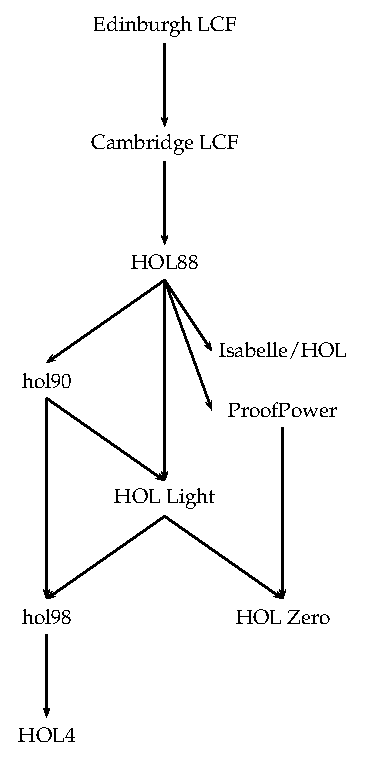
\includegraphics[width=3.2cm]{images/hol-family}
\end{column}
\end{columns}

\end{frame}

%%% Local Variables:
%%% mode: latex
%%% TeX-master: "hol"
%%% End:
